\documentclass{beamer}
\usepackage{graphicx}

\newcommand*{\rom}[1]{\expandafter\@slowromancap\romannumeral #1@}
\newcommand{\ts}{\textsuperscript}


\usetheme{Boadilla}

% items enclosed in square brackets are optional; explanation below
\title[Privacy in Art, Books, and Film]{I've Got Nothing to Hide: \\
  Exploring Privacy in Art, Books, and Film}
\author[Josh Datko]{Joshua Datko}
\institute[Drexel]{
  Department of Computer Science\\
  Drexel University\\
  Philadelphia, PA 19103\\[1ex]
  \texttt{jbd65@drexel.edu}
}
\date[September 2013]{September 28, 2013}

\setbeamertemplate{bibliography item}[text]




\begin{document}

%--- the titlepage frame -------------------------%
\begin{frame}[plain]
  \titlepage
\end{frame}

\begin{frame}
  \frametitle{I've Got Nothing to Hide}

A brief summary of \emph{``I've Got Nothing to Hide'' and Other
  Misunderstandings of Privacy} by Daniel J. Solove.

\begin{itemize}
\item If you have nothing to hide, what do you have to fear?
\item More like, ``I don't care what happens, so long as it doesn't
  happen to me.''
\item Strongest argument has a utilitarian perspective: national
  security is more important than my privacy.

\end{itemize}
\end{frame}


\begin{frame}

\frametitle{Privacy is hard to define}

The taxonomy of privacy:

\begin{columns}[c] % the "c" option specifies center vertical alignment
    \column{.5\textwidth} % column designated by a command

    \begin{itemize}
    \item Information Collection
      \begin{itemize}
      \item Surveillance
      \item Interrogation
      \end{itemize}
    \item Information Processing
      \begin{itemize}
      \item Aggregation
      \item Identification
      \item Insecurity
      \item Secondary Use
      \item Exclusion
      \end{itemize}

    \end{itemize}


    \column{.5\textwidth}

    \begin{itemize}
    \item Information Dissemination
      \begin{itemize}
      \item Breach of Confidentiality
      \item Disclosure
      \item Exposure
      \item Increased Accessibility
      \item Blackmail
      \item Appropriation
      \item Distortion
        \end{itemize}
    \item Invasion
      \begin{itemize}
      \item Intrusion
      \item Decisional Interference

        \end{itemize}

      \end{itemize}

    \end{columns}


\end{frame}



\begin{frame}

\begin{columns}[c] % the "c" option specifies center vertical alignment
    \column{.5\textwidth} % column designated by a command

    \begin{block}{}
      Privacy in Art.
    \end{block}


    \column{.5\textwidth}

    \end{columns}


\end{frame}



\begin{frame}

\frametitle{\emph{The Neighbors} (2013) by Arne Svenson}

\begin{itemize}
\item Photographer takes pictures of his neighbors, without their
  knowledge,  in Tribeca (NYC).
\item Two neighbors sued.  Their children were in the photos.
\item Court ruled the artist was protected under the First Amendment.


\end{itemize}

\begin{block}{I have nothing to hide.}
    Unless you take a picture of me and call it art!
  \end{block}

\end{frame}

\begin{frame}
\frametitle{\emph{Neighbors}}


    \begin{columns}[c] % the "c" option specifies center vertical alignment
    \column{.5\textwidth} % column designated by a command
    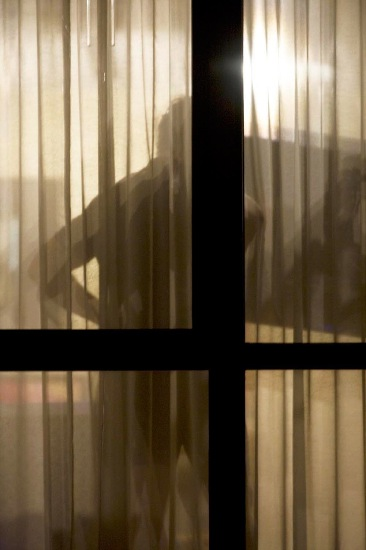
\includegraphics[width=\textwidth,height=0.8\textheight,keepaspectratio]{img/10_website_IMG_4763}

    \column{.5\textwidth}
    \begin{figure}
    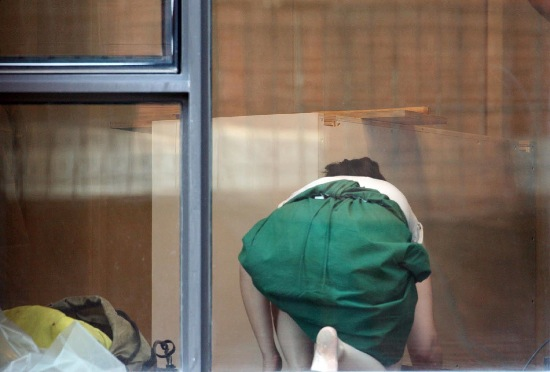
\includegraphics[width=\textwidth,height=0.8\textheight,keepaspectratio]{img/4_website_IMG_3013.jpg}
    \caption{Photos Copyright Arne Svenson}
    \end{figure}

    \end{columns}


\end{frame}

\begin{frame}
\frametitle{Face to Facebook}

Stealing 1 million Facebook profiles, filtering them with face-recognition software, and then,
posting them on a custom-made dating website, sorted by their facial
expressions characteristics.

\begin{columns}[c] % the "c" option specifies center vertical alignment
    \column{.5\textwidth} % column designated by a command
    \begin{itemize}
    \item All ``singles'' were involuntarily added to a fake an
      experimental dating site.
    \item Let's watch the introduction video.
    \item Great example of \emph{secondary usage}

    \end{itemize}

    \column{.5\textwidth}
    \begin{figure}
    \includegraphics[width=\textwidth,height=0.4\textheight,keepaspectratio]{img/fbFaces}
    \caption{Facebook Faces by Joern Roeder and Jonathan Pirnay,
      University of Visual Arts and Design Kassel, Germany, 2011}

    \end{figure}

    \end{columns}



\end{frame}


\begin{frame}

\begin{columns}[c] % the "c" option specifies center vertical alignment
    \column{.5\textwidth} % column designated by a command

    \begin{block}{}
      Privacy in Fiction.
    \end{block}


    \column{.5\textwidth}

    \end{columns}


\end{frame}


\begin{frame}
\frametitle{\emph{The Trial} by Franz Kafka}

\begin{itemize}
\item Referred to by the author as an example that ``depicts a
  bureaucracy with insrutable purposes that uses people's information
  to make important decisions about them, yet denies the people the
  ability to participate in how their information is used.''

\item Reading from beginning of \emph{The Trial}.
\item Reading from \emph{Harper's}, September 2013, \emph{Life as a
  Terrorist: Uncovering my FBI File} by William T. Vollmann
\end{itemize}

\begin{block}{I have nothing to hide.}
    But when the government hides information about you, it enables a
    sense of frustration and powerlessness.
  \end{block}


\end{frame}


\begin{frame}
\frametitle{\emph{Little Brother} and \emph{Homeland} by Cory
  Doctorow}

\begin{columns}[c] % the "c" option specifies center vertical alignment
    \column{.5\textwidth} % column designated by a command
    \begin{itemize}
    \item Cory Doctorow: EFF, Boing Boing, several books.
    \item The day after tomorrow setting: terrorist attack San Francisco.
    \item \emph{Little Brother} teaches you how to have a GPG Signing
      party and how to run anonymizing software (like Tails and Tor).
    \item Afterwards by Bruce Schneier, Andrew Huang, Jacob Appelbaum,
      Aaron Schwartz.
    \item \emph{Little Brother} has an \emph{excellent} Bibliography for
      other readings on security.
    \end{itemize}


    \column{.5\textwidth}
    \begin{figure}
    
\includegraphics[width=\textwidth,height=0.8\textheight,keepaspectratio]{img/Little-Brother}

    \end{figure}

    \end{columns}



\end{frame}

\begin{frame}

\begin{columns}[c] % the "c" option specifies center vertical alignment
    \column{.5\textwidth} % column designated by a command

    \begin{block}{}
      Privacy in Film.
    \end{block}


    \column{.5\textwidth}

    \end{columns}


\end{frame}


\begin{frame}
\frametitle{\emph{V for Vendetta} 2005}

\begin{columns}[c] % the "c" option specifies center vertical alignment
    \column{.5\textwidth} % column designated by a command
    \begin{itemize}

      \item Orwellian: state surveillance, mandatory curfews, state media.
      \item Popularized Guy Fawkes Masks.
      \item Banned books, art, and subversive material.
    \end{itemize}

    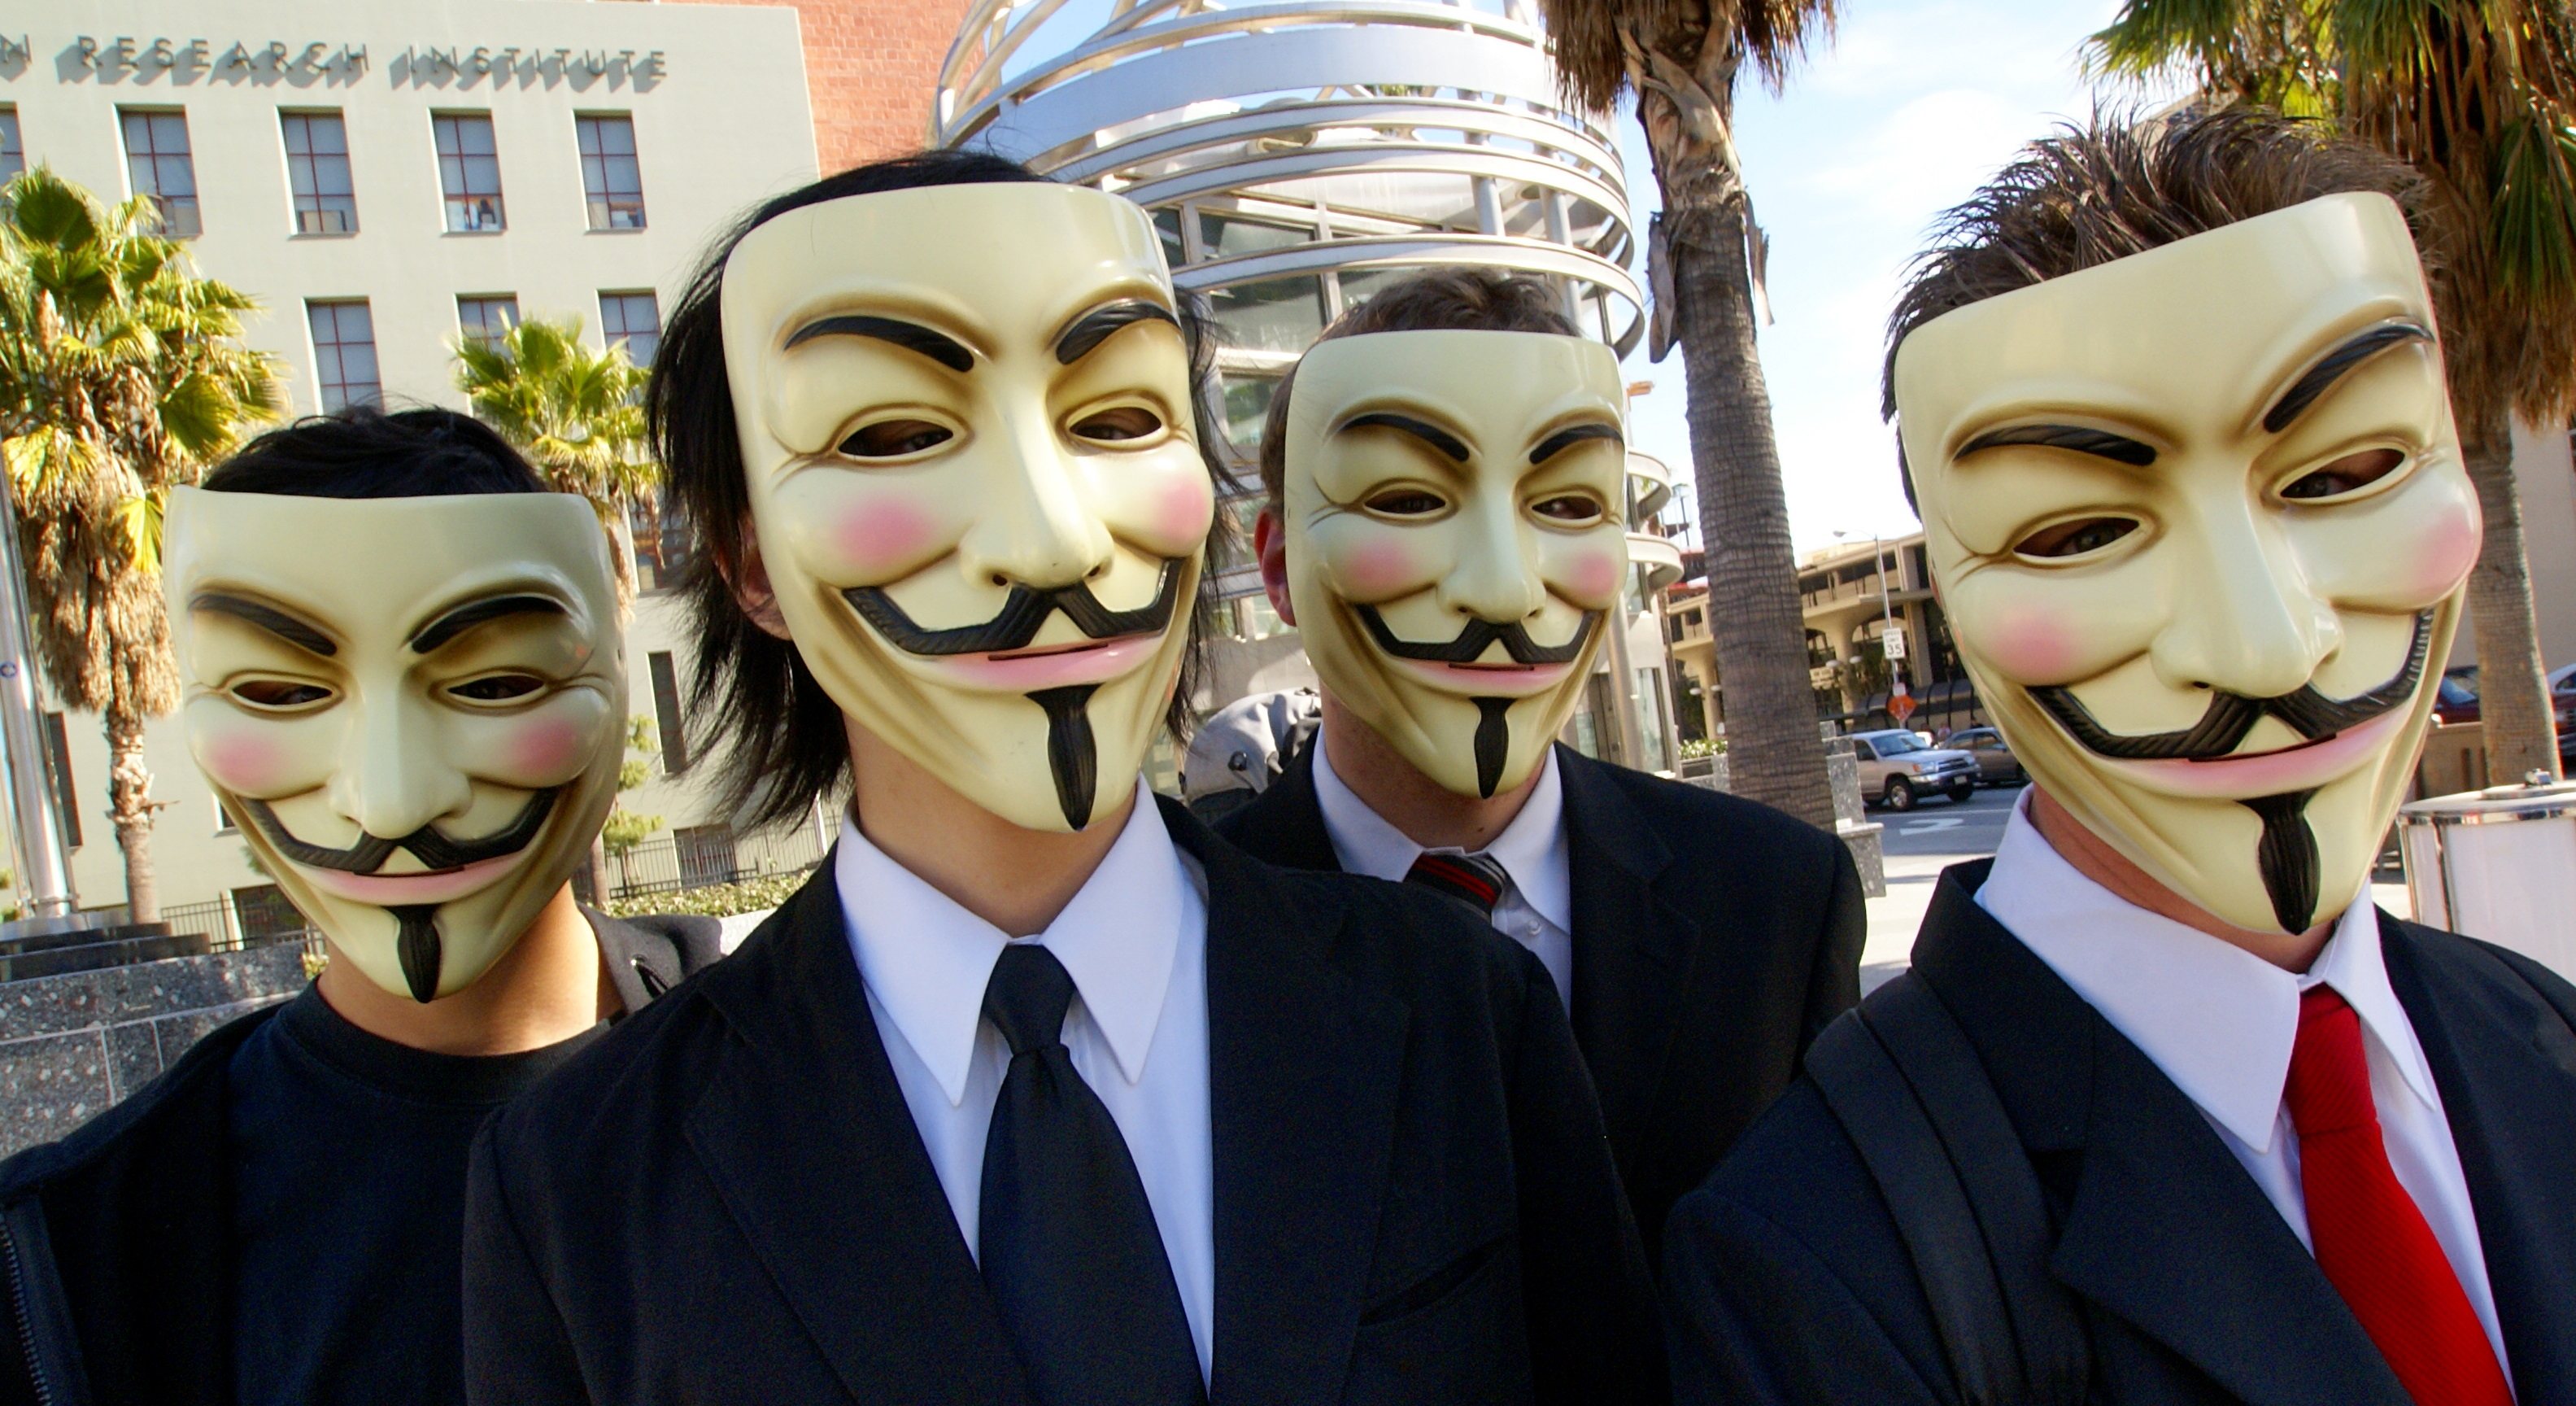
\includegraphics[width=\textwidth,height=0.6\textheight,keepaspectratio]{img/guy_fawkes}

    \column{.5\textwidth}
    \begin{figure}
    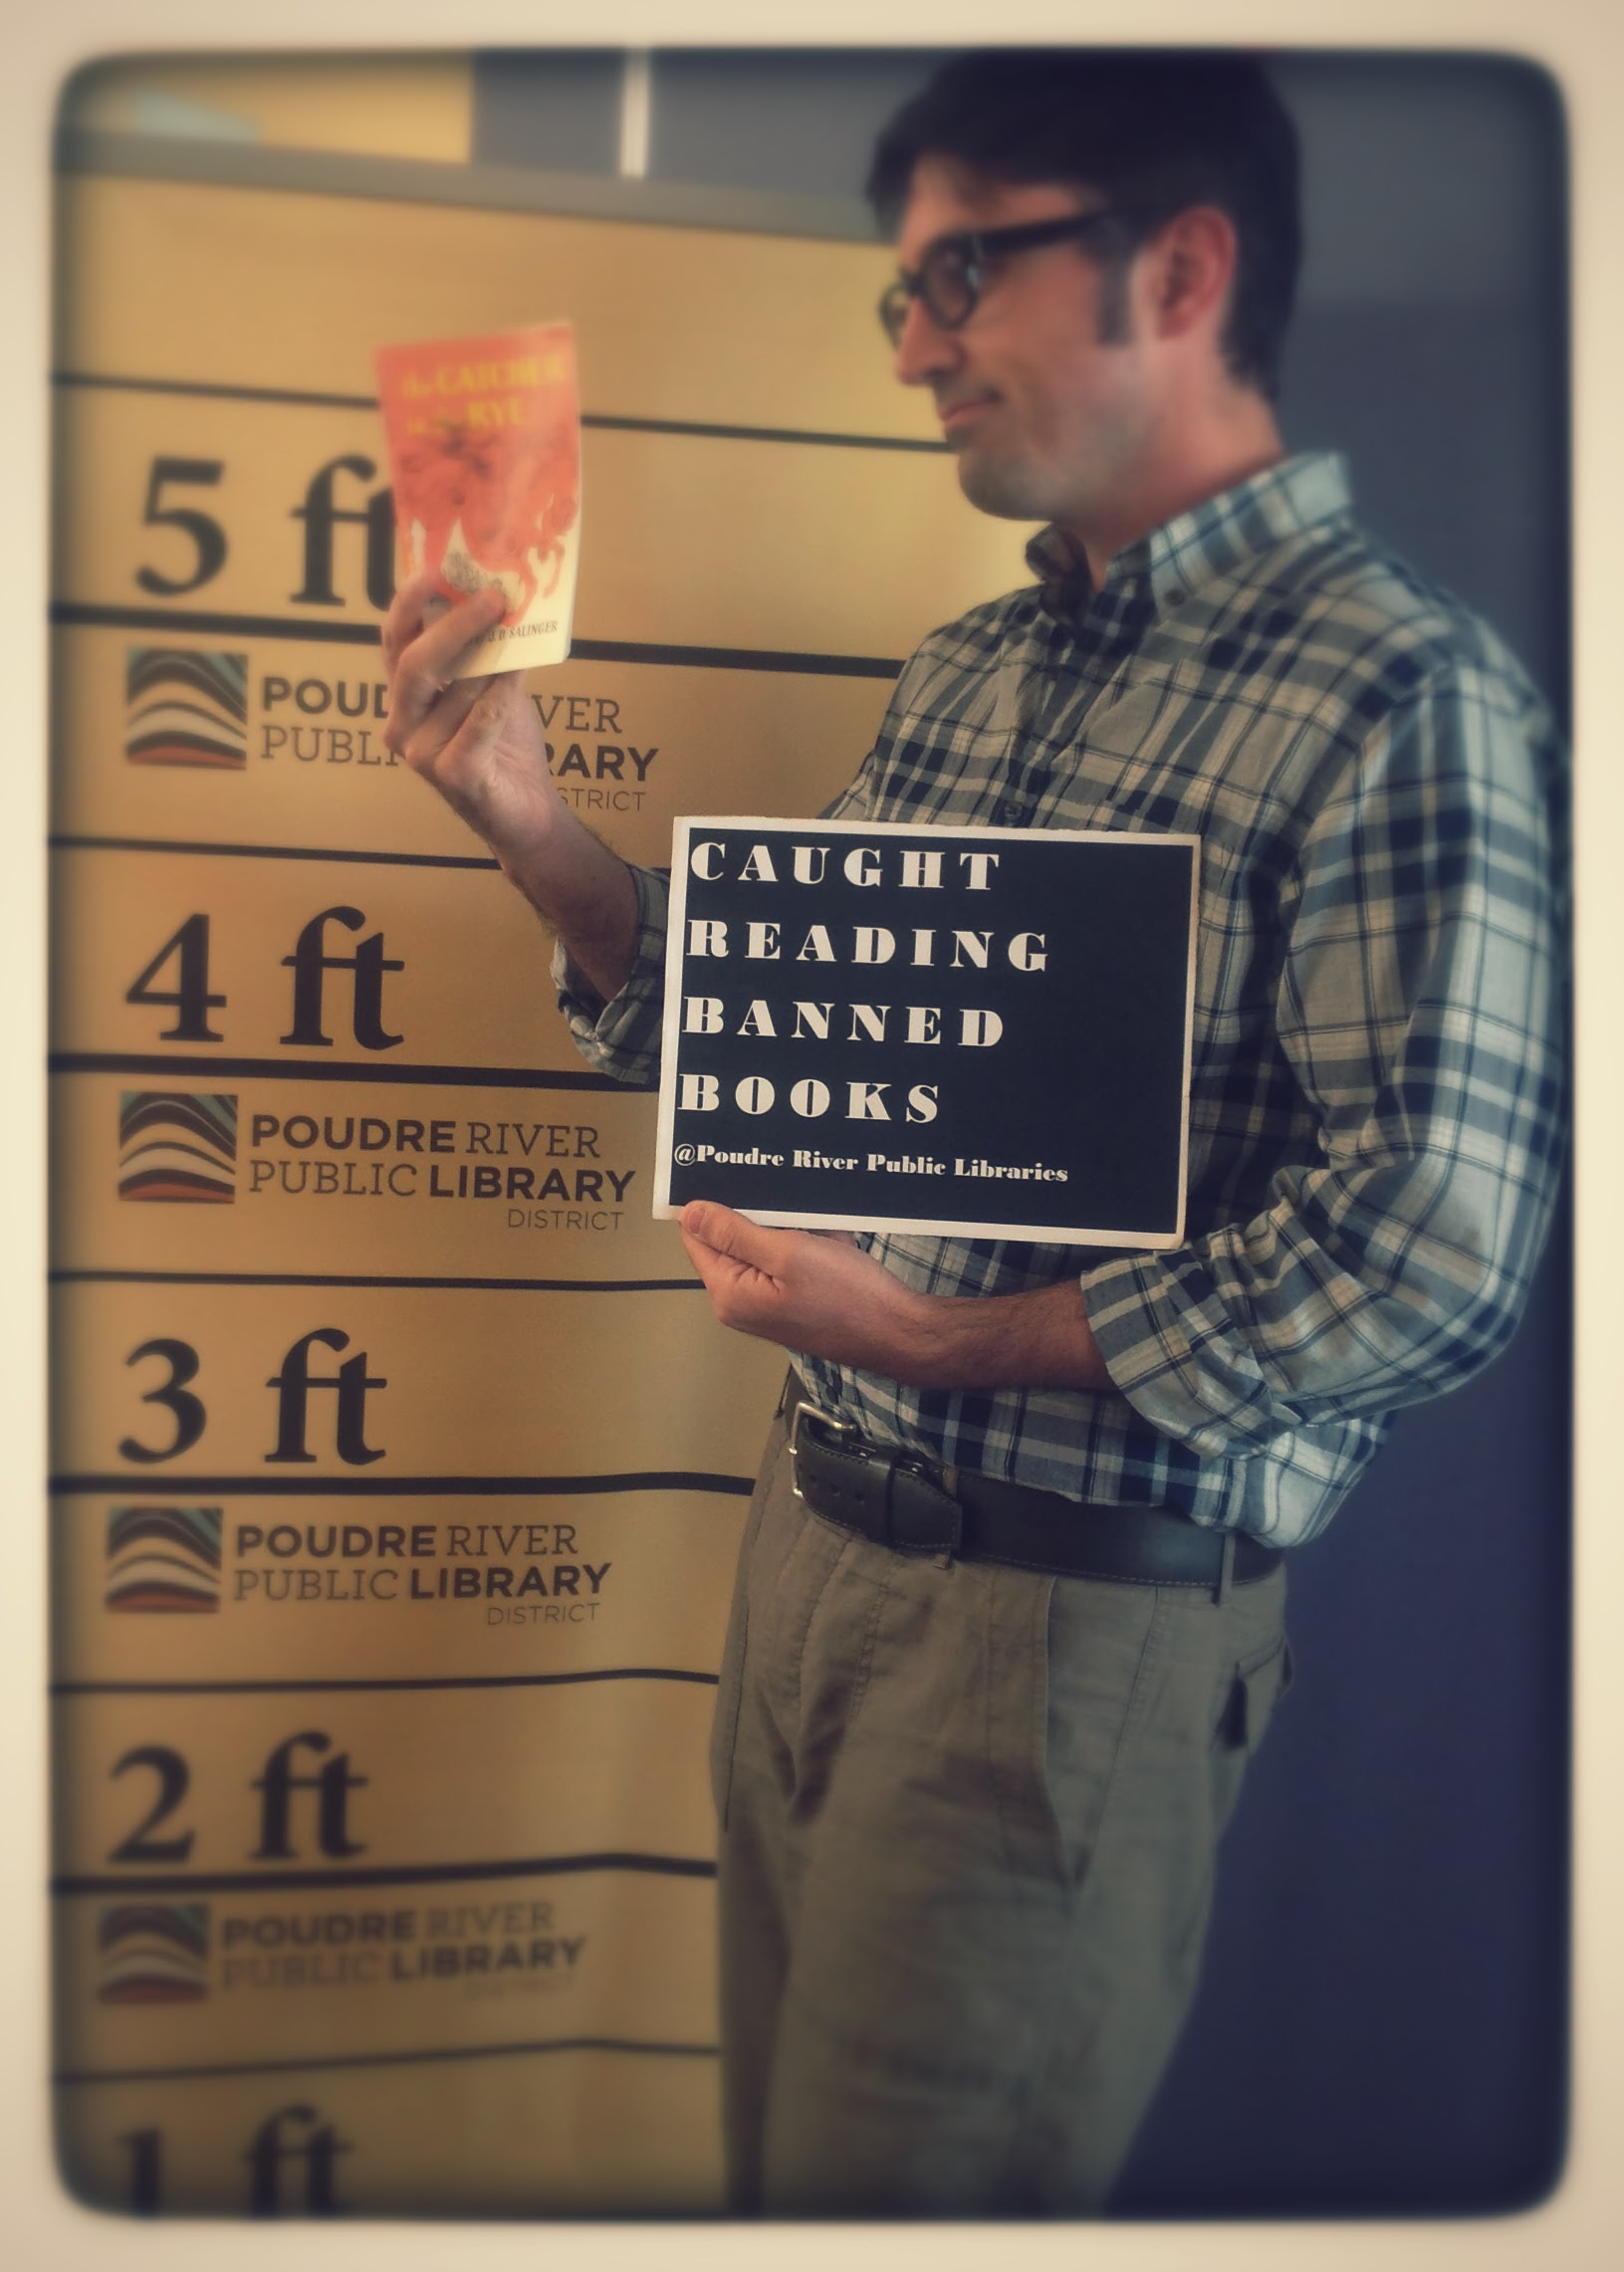
\includegraphics[width=\textwidth,height=0.6\textheight,keepaspectratio]{img/banned_books}
    %\caption{Me reading a banned book.  I would not do well in a
      %\emph{V for Vendetta} world.}
    \begin{block}{Caught with a banned book}
      I would not do well in a \emph{V for Vendetta} world.
    \end{block}
    \end{figure}

    \end{columns}




\end{frame}

\begin{frame}
\frametitle{\emph{Das Leben der Anderen} (2006)}
\begin{columns}[c] % the "c" option specifies center vertical alignment
    \column{.5\textwidth} % column designated by a command
    \begin{itemize}

      \item 1950 - 1990 during the DDR, a \emph{real} surveillance
        state existed.
      \item Nearly every item on the taxonomy of privacy is violated.
      \item Stasi infiltration ran deep: industry, schools, and spouses.
    \end{itemize}

    \column{.5\textwidth}
    \begin{figure}
    
\includegraphics[width=\textwidth,height=0.6\textheight,keepaspectratio]{img/stasi}
    %\caption{Me reading a banned book.  I would not do well in a
      %\emph{V for Vendetta} world.}


    \end{figure}

    \end{columns}

\begin{block}{Why invent dystopias?}
      History serves as a better example.
\end{block}


\end{frame}

\begin{frame}
\frametitle{Discussion Ideas}

\begin{itemize}
\item Would you keep your blinds open in NYC if you lived there?  What
  if your neighbor was taking pictures?
\item When, if ever, would you consider filling a Freedom of
  Information Act (FOIA) request for your file?
\item The TSA back-scatter machines have raised privacy concerns
  because of the revealing images.  Would you / did you go throw them?
  Did you feel any pressure to choose the scanner over the pat-down?

\end{itemize}

\end{frame}


\end{document}

%%% Local Variables:
%%% mode: latex
%%% TeX-master: t
%%% End:
